\documentclass[11pt]{article}
\usepackage[english,vietnam]{babel}
\usepackage[utf8]{inputenc}

\usepackage{a4wide,amssymb,epsfig,latexsym,multicol,array,hhline,fancyhdr}
\usepackage{lastpage}
\usepackage{enumerate}
\usepackage{color}
\usepackage{graphicx}
\usepackage{array}
\usepackage{tabularx}
\usepackage{multirow}
\usepackage{multicol}
\usepackage{rotating}
\usepackage{graphics}
\usepackage{geometry}
\usepackage{setspace}
\usepackage{epsfig}
\usepackage{tikz}
\usepackage{placeins}
\usepackage{appendix}
\usepackage{booktabs}
\usetikzlibrary{arrows,snakes,backgrounds}

\begin{document}
	\begin{titlepage}		
		\begin{flushleft}
		\noindent Trường Đai Học Bách Khoa Tp. Hồ Chí Minh\\
		Khoa Khoa Học \& Kỹ Thuật Máy Tính\\
		\end{flushleft}
		
		\vspace{1cm}
		
		\begin{figure}[h!]
		\begin{center}
		
\includegraphics[width=30mm]{hcmut.png}
		\end{center}
		\end{figure}
		
		\vspace{1cm}
		
		
		\begin{center}
	
		\textbf{{\Huge HƯỚNG DẪN SỬ DỤNG PHẦN MỀM HỖ TRỢ SẮP LỊCH }}\\
	
		\end{center}
		
		\vspace{4cm}
	
		\begin{flushright}
			Người thực hiện:\\
			Nguyễn Quốc Thịnh
		\end{flushright}
	\end{titlepage}
	% % % % % % % % % % % % % % % % % % % % % % %
	\tableofcontents 
	\newpage
	\section{Giới thiệu}
	Phần mềm bước đầu đang cố gắng đưa ra một cách chuẩn hóa dữ liệu. Thông qua việc sử dụng các mẫu đã có định dạng sẵn, chúng ta sẽ sử dụng chương trình để tính toán tự động một số thông số đơn giản ban đầu.\\
	Bước phát triển tiếp theo của phần mềm là cố gắng hạn chế việc nhập liệu bằng tay trong nhiều công đoạn và lưu trữ dữ liệu một cách có cấu trúc và bền vững.\\
	Mục tiêu cuối cùng hướng đến đó là phần mềm có khả năng hỗ trợ ra quyết định cho người dùng.\\
	Chương trình gồm có 2 giai đoạn:
	\begin{itemize}
		\item Giai đoạn 1: đọc file lịch chiếu cũ, tạo ra file sản lượng mẫu.
		\item Giai đoạn 2: đọc file lịch chiếu cũ, file sản lượng đã được điền đầy đủ các thông tin và file định dạng cho file đánh giá độ hiệu quả. Cuối cùng đưa ra file đánh giá kết quả trình chiếu.
	\end{itemize}	
	% % % % % % % % % % % % % % % % % % % % % % %
	\section{Các mẫu dữ liệu đầu vào}
	Dữ liệu đầu vào gồm có:
	\begin{itemize}
		\item File lịch trình chiếu mẫu
		\item File sản lượng mẫu
		\item File định dạng cho file đánh giá kết quả trình chiếu
	\end{itemize}
	Các file mẫu này được đính kèm theo tài liệu này.
	\subsection{Lịch trình chiếu}
	Lịch trình chiếu giống như lịch trình chiếu đã dùng. Cách đặt tên cho sheet cũng như cũ. Xem file mẫu "Schedule-Standard.xlsx".\\
	Tuy nhiên có một số lưu ý:
	\begin{itemize}
		\item Nội dung lịch trình bắt đầu ngay từ cột A, không để cột A trống
		\item Tên của sheet có định dạng $d_{1}d_{1}-d_{2}d_{2}.mm$ với $d_{1}d_{1}$ là ngày bắt đầu $d_{2}d_{2}$ là ngày cuối, $mm$ là tháng.
		\item Trong trường hợp ngày bắt đầu và kết thúc nằm giữa 2 tháng thì chúng là kí hiệu $\&$
		\item Không cần ghi năm trong tên sheet, chỉ ghi năm trong phần tiêu đề mà thôi.
		\item Phần mềm chỉ làm việc với sheet cuối cùng của file lịch trình chiếu.\\
		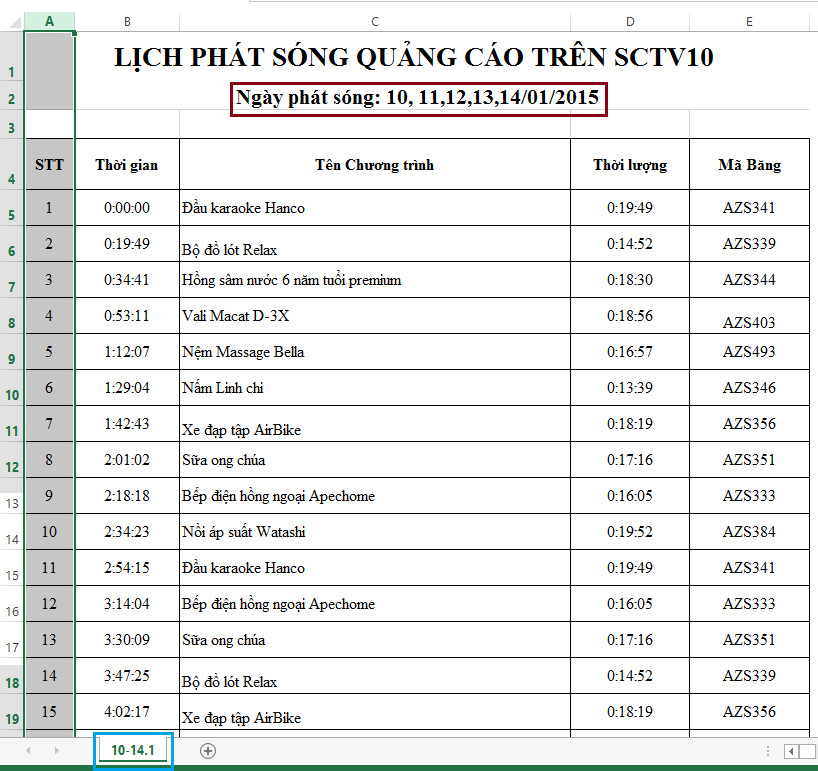
\includegraphics[width=130mm]{im1.png}
	\end{itemize}
	\subsection{File sản lượng}
	File sản lượng mẫu "Product-Quantity-Standard.xlsx" sẽ gồm 2 nhóm thông tin:
	\begin{itemize}
		\item Thông tin đã rút trích được từ file lịch trình chiếu cũ
		\begin{itemize}
			\item Mã chương trình, tên chương trình, thời lượng, tần số phát
		\end{itemize}
		\item Thông tin còn thiếu cần được cung cấp
		\begin{itemize}
			\item Category, giá sản phẩm quảng cáo trong chương trình
			\item Group đã được đánh giá trong file efficiency trước đây
			\item Sản lượng: sản lượng cần cung cấp theo từng ngày theo như file mẫu\\
			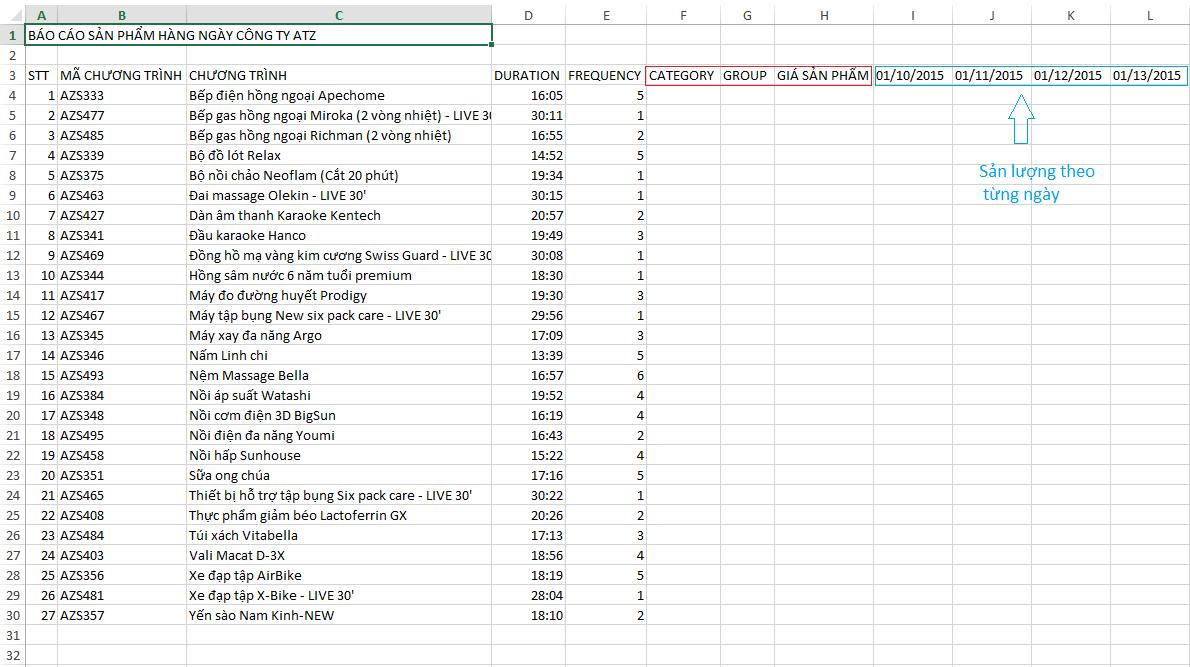
\includegraphics[width=140mm]{im2.png}
			\item Các cột sản lượng không nhất thiết phải điền hết, chương trình chỉ tính cho các cột có giá trị, tuy nhiên hiện tại các cột này phải liên tục. Xin xem file mẫu "Product-Quantity-Standard-FullData.xlsx"
		\end{itemize}
	\end{itemize}
	%%%%%%%%%%%%%%%%%%%%%%%%%%%%%%%%%%%%%%%%%%%%%%%%%%%%%
	\subsection{File định dạng cho file đánh giá độ hiệu quả}	
	File định dạng mẫu giúp người dùng có thể dễ dàng thay đổi màu sắc, font, cở chữ, màu của các cột trong file dánh giá độ hiệu quả. File mẫu là "TemplateEfficiency.xlsx"
	\newpage
	%%%%%%%%%%%%%%%%%%%%%%%%%%%%%%%%%%%%%%%%%%%%%%%%%%%%%
	\section{Các bước sử dụng phần mềm}
	\subsection{Cấu hình hỗ trở}
	Phần mềm chạy tốt trên Win7 và Win8.1. Để chạy chương trình cần có thư viện Microsoft .NET Framework 4 (Standalone Installer).\\
	Link download: http://www.microsoft.com/en-us/download/details.aspx?id=17718
	\subsection{Bước đầu tiên}
	Chúng ta chọn nút "Search" để tìm kiếm file lịch trình chiếu cũ.\\
	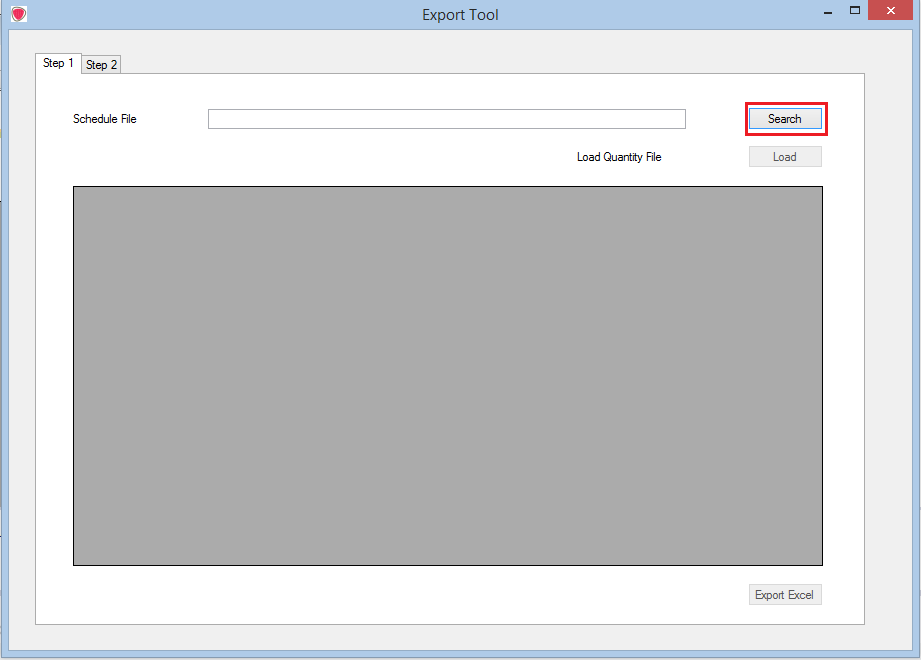
\includegraphics[width=140mm]{im3.png}\\
	Đọc dữ liệu\\
	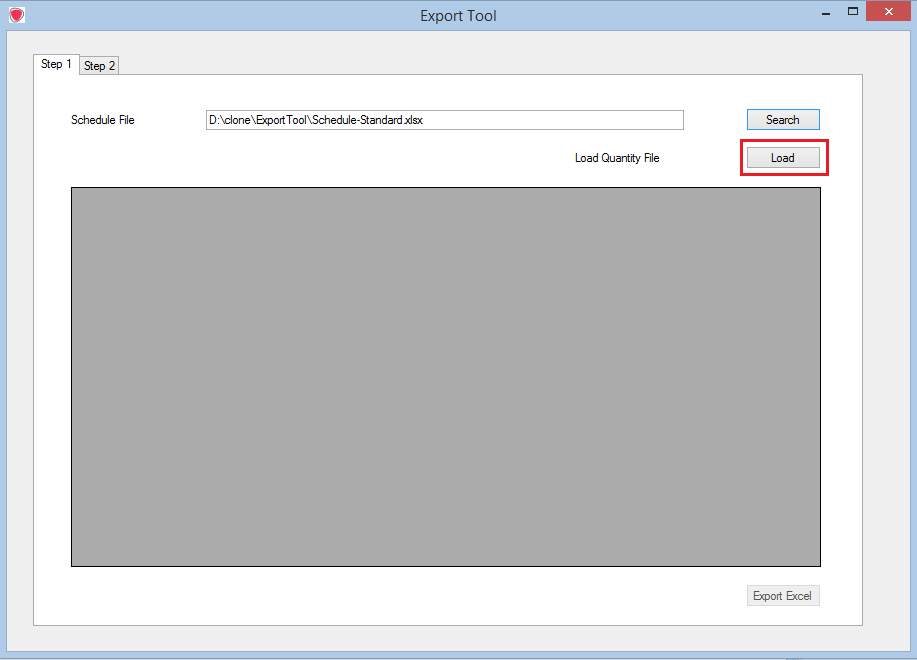
\includegraphics[width=140mm]{im4.png}\\
	Lưu file sản lượng mẫu\\
	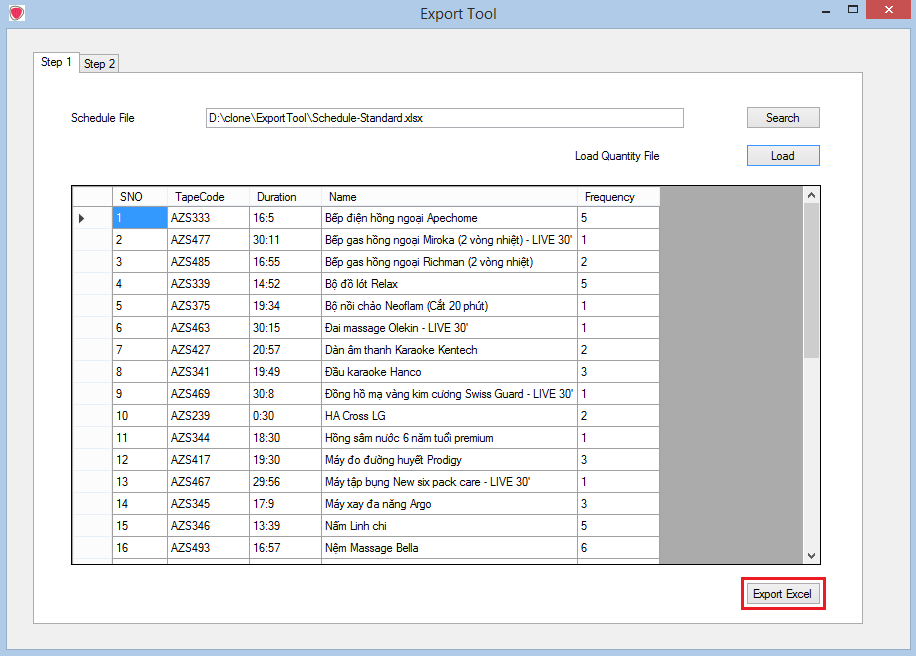
\includegraphics[width=140mm]{im5.png}\\
	\subsection{Bước thứ 2}
	Kết thúc bước đầu tiên chúng ta có file sản lượng mẫu. Người dùng hoàn thành các thông tin còn thiếu trong file sản lượng. Sau khi có đầy đủ dữ liệu chúng ta chuyển qua bước 2.\\
	Tìm các file cần thiết: lịch trình chiếu cũ, file sản lượng đã điền thông tin, file định dạng.\\
	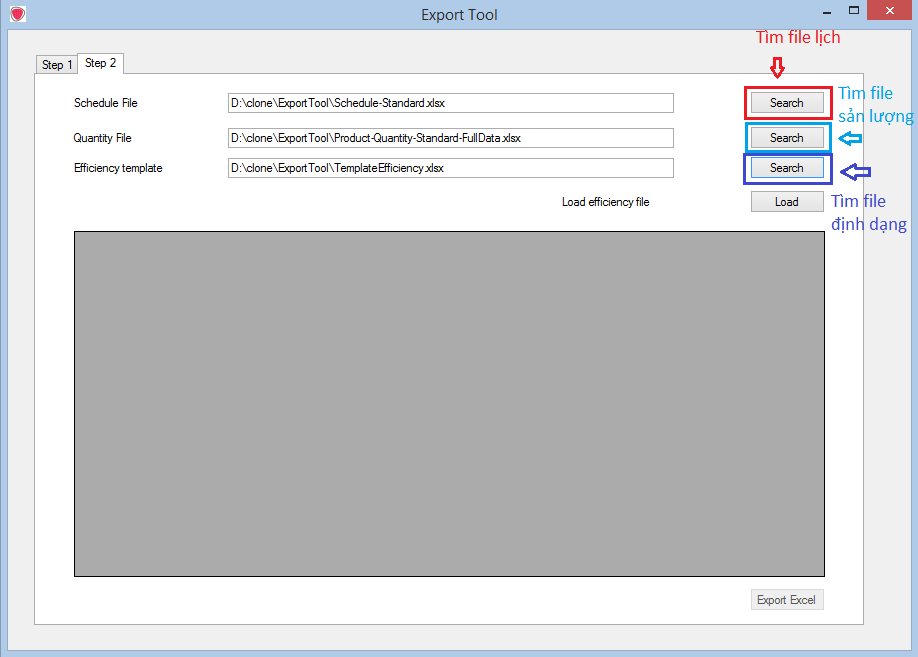
\includegraphics[width=140mm]{im6.png}\\
	Đọc dữ liệu\\
	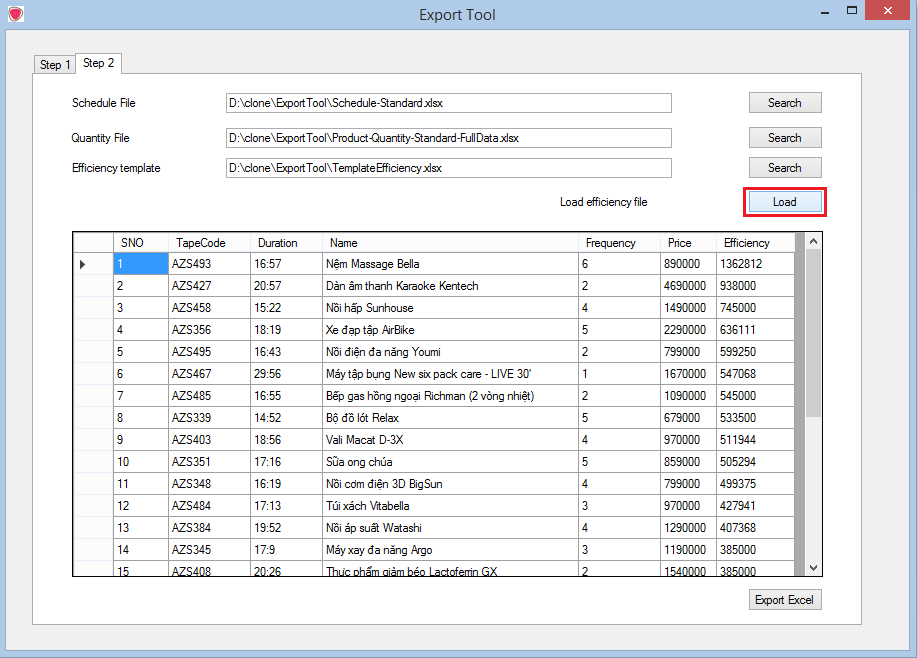
\includegraphics[width=140mm]{im7.png}\\
	Lưu lại file đánh giá độ hiệu quả\\
	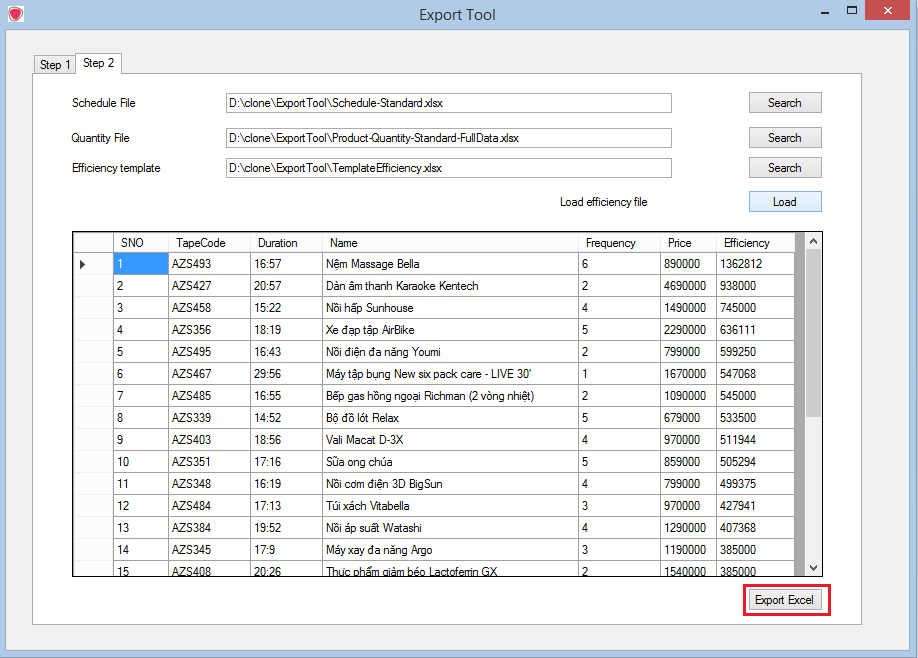
\includegraphics[width=140mm]{im8.png}\\
%%%%%%%%%%%%%%%%%%%%%%%%%%%%%%%%%%%%%%%%%%%%%%%%%%%%%%%%	
	\section{Liên hệ}
	Mọi ý kiến đóng góp xin liên hệ:\\
	Nguyễn Quốc Thịnh\\
	Email: nqt900@gmail.com\\
	Skype: nqthinh90
	
\end{document}


%%%%%%%%%%%%%%%

\end{document}


